
%(BEGIN_QUESTION)
% Copyright 2007, Tony R. Kuphaldt, released under the Creative Commons Attribution License (v 1.0)
% This means you may do almost anything with this work of mine, so long as you give me proper credit

Suppose you see this process response following a manual ``step-change'' in the output (final control element):

$$\includegraphics[width=15.5cm]{i01663x01.eps}$$

Is this process inherently {\it self-regulating}, or {\it integrating}?  Explain your answer.

\underbar{file i01663}
%(END_QUESTION)





%(BEGIN_ANSWER)

This is an {\it integrating} process.  We know this because the process variable (PV) does not reach equilibrium after the output perturbation.  Rather, it ``integrates'' onward to full-scale saturation over time, with little sign of stabilizing.

%(END_ANSWER)





%(BEGIN_NOTES)


%INDEX% Control, process characteristics: self-regulating versus integrating

%(END_NOTES)


